\ProvidesFile{themes/space/theme.tex}[2026/09/27 Space poster theme]

\RequirePackage{tgtermes}
\RequirePackage[most]{tcolorbox}

% ====================
% Theme tokens
% ====================

\definecolor{SpaceInk}{HTML}{031426}
\definecolor{SpacePanel}{HTML}{061C31}
\definecolor{SpaceFooter}{HTML}{0C122B}
\definecolor{SpaceCream}{HTML}{F4EBD8}
\definecolor{SpaceCyan}{HTML}{73E5FF}
\definecolor{SpaceBlue}{HTML}{21A8E0}
\definecolor{SpaceGold}{HTML}{FFD49B}
\definecolor{SpaceMuted}{HTML}{AEC4D4}
\definecolor{SpaceViolet}{HTML}{BA83E6}

\colorlet{CrispWhite}{SpacePanel}
\colorlet{DarkNavy}{SpaceInk}
\colorlet{Aqua}{SpaceCyan}
\colorlet{SkyBlue}{SpaceBlue}
\colorlet{TakeawayAccent}{SpaceGold}
\colorlet{SoftGray}{SpaceMuted}

\setbeamercolor{normal text}{fg=SpaceCream,bg=}
\setbeamercolor{structure}{fg=SpaceCyan}
\setbeamercolor{item}{fg=SpaceCyan}
\setbeamercolor{headline}{fg=SpaceCream,bg=}
\setbeamercolor{headline title}{fg=SpaceCream,bg=}
\setbeamercolor{headline author}{fg=SpaceCream,bg=}
\setbeamercolor{headline institute}{fg=SpaceCream,bg=}
\setbeamercolor{block title}{fg=SpaceCream,bg=}
\setbeamercolor{block body}{fg=SpaceCream,bg=}
\setbeamercolor{block alerted title}{fg=SpaceCream,bg=}
\setbeamercolor{block alerted body}{fg=SpaceCream,bg=}
\setbeamercolor{caption name}{fg=SpaceCyan}
\setbeamercolor{caption}{fg=SpaceCream}
\setbeamercolor{space footer}{fg=SpaceCream,bg=SpaceFooter}
\setbeamercolor{space footer rule}{bg=SpaceCyan}

\usefonttheme{serif}
\setbeamerfont{normal text}{family=\rmfamily,size=\large}
\setbeamerfont{headline title}{family=\rmfamily,size=\Huge,series=\bfseries}
\setbeamerfont{headline author}{family=\rmfamily,size=\Large}
\setbeamerfont{headline institute}{family=\rmfamily,size=\large}
\setbeamerfont{block title}{family=\rmfamily,size=\Large,series=\bfseries}
\setbeamerfont{block body}{family=\rmfamily,size=\large}
\setbeamerfont{itemize/enumerate body}{family=\rmfamily,size=\large}
\setbeamerfont{itemize/enumerate subbody}{family=\rmfamily,size=\normalsize}
\setbeamerfont{caption}{family=\rmfamily,size=\normalsize}
\setbeamerfont{footline}{family=\rmfamily,size=\normalsize}

% ====================
% Background
% ====================

\setbeamertemplate{background}{%
  \begin{tikzpicture}[remember picture,overlay]
    \node[inner sep=0pt] at (current page.center) {%
      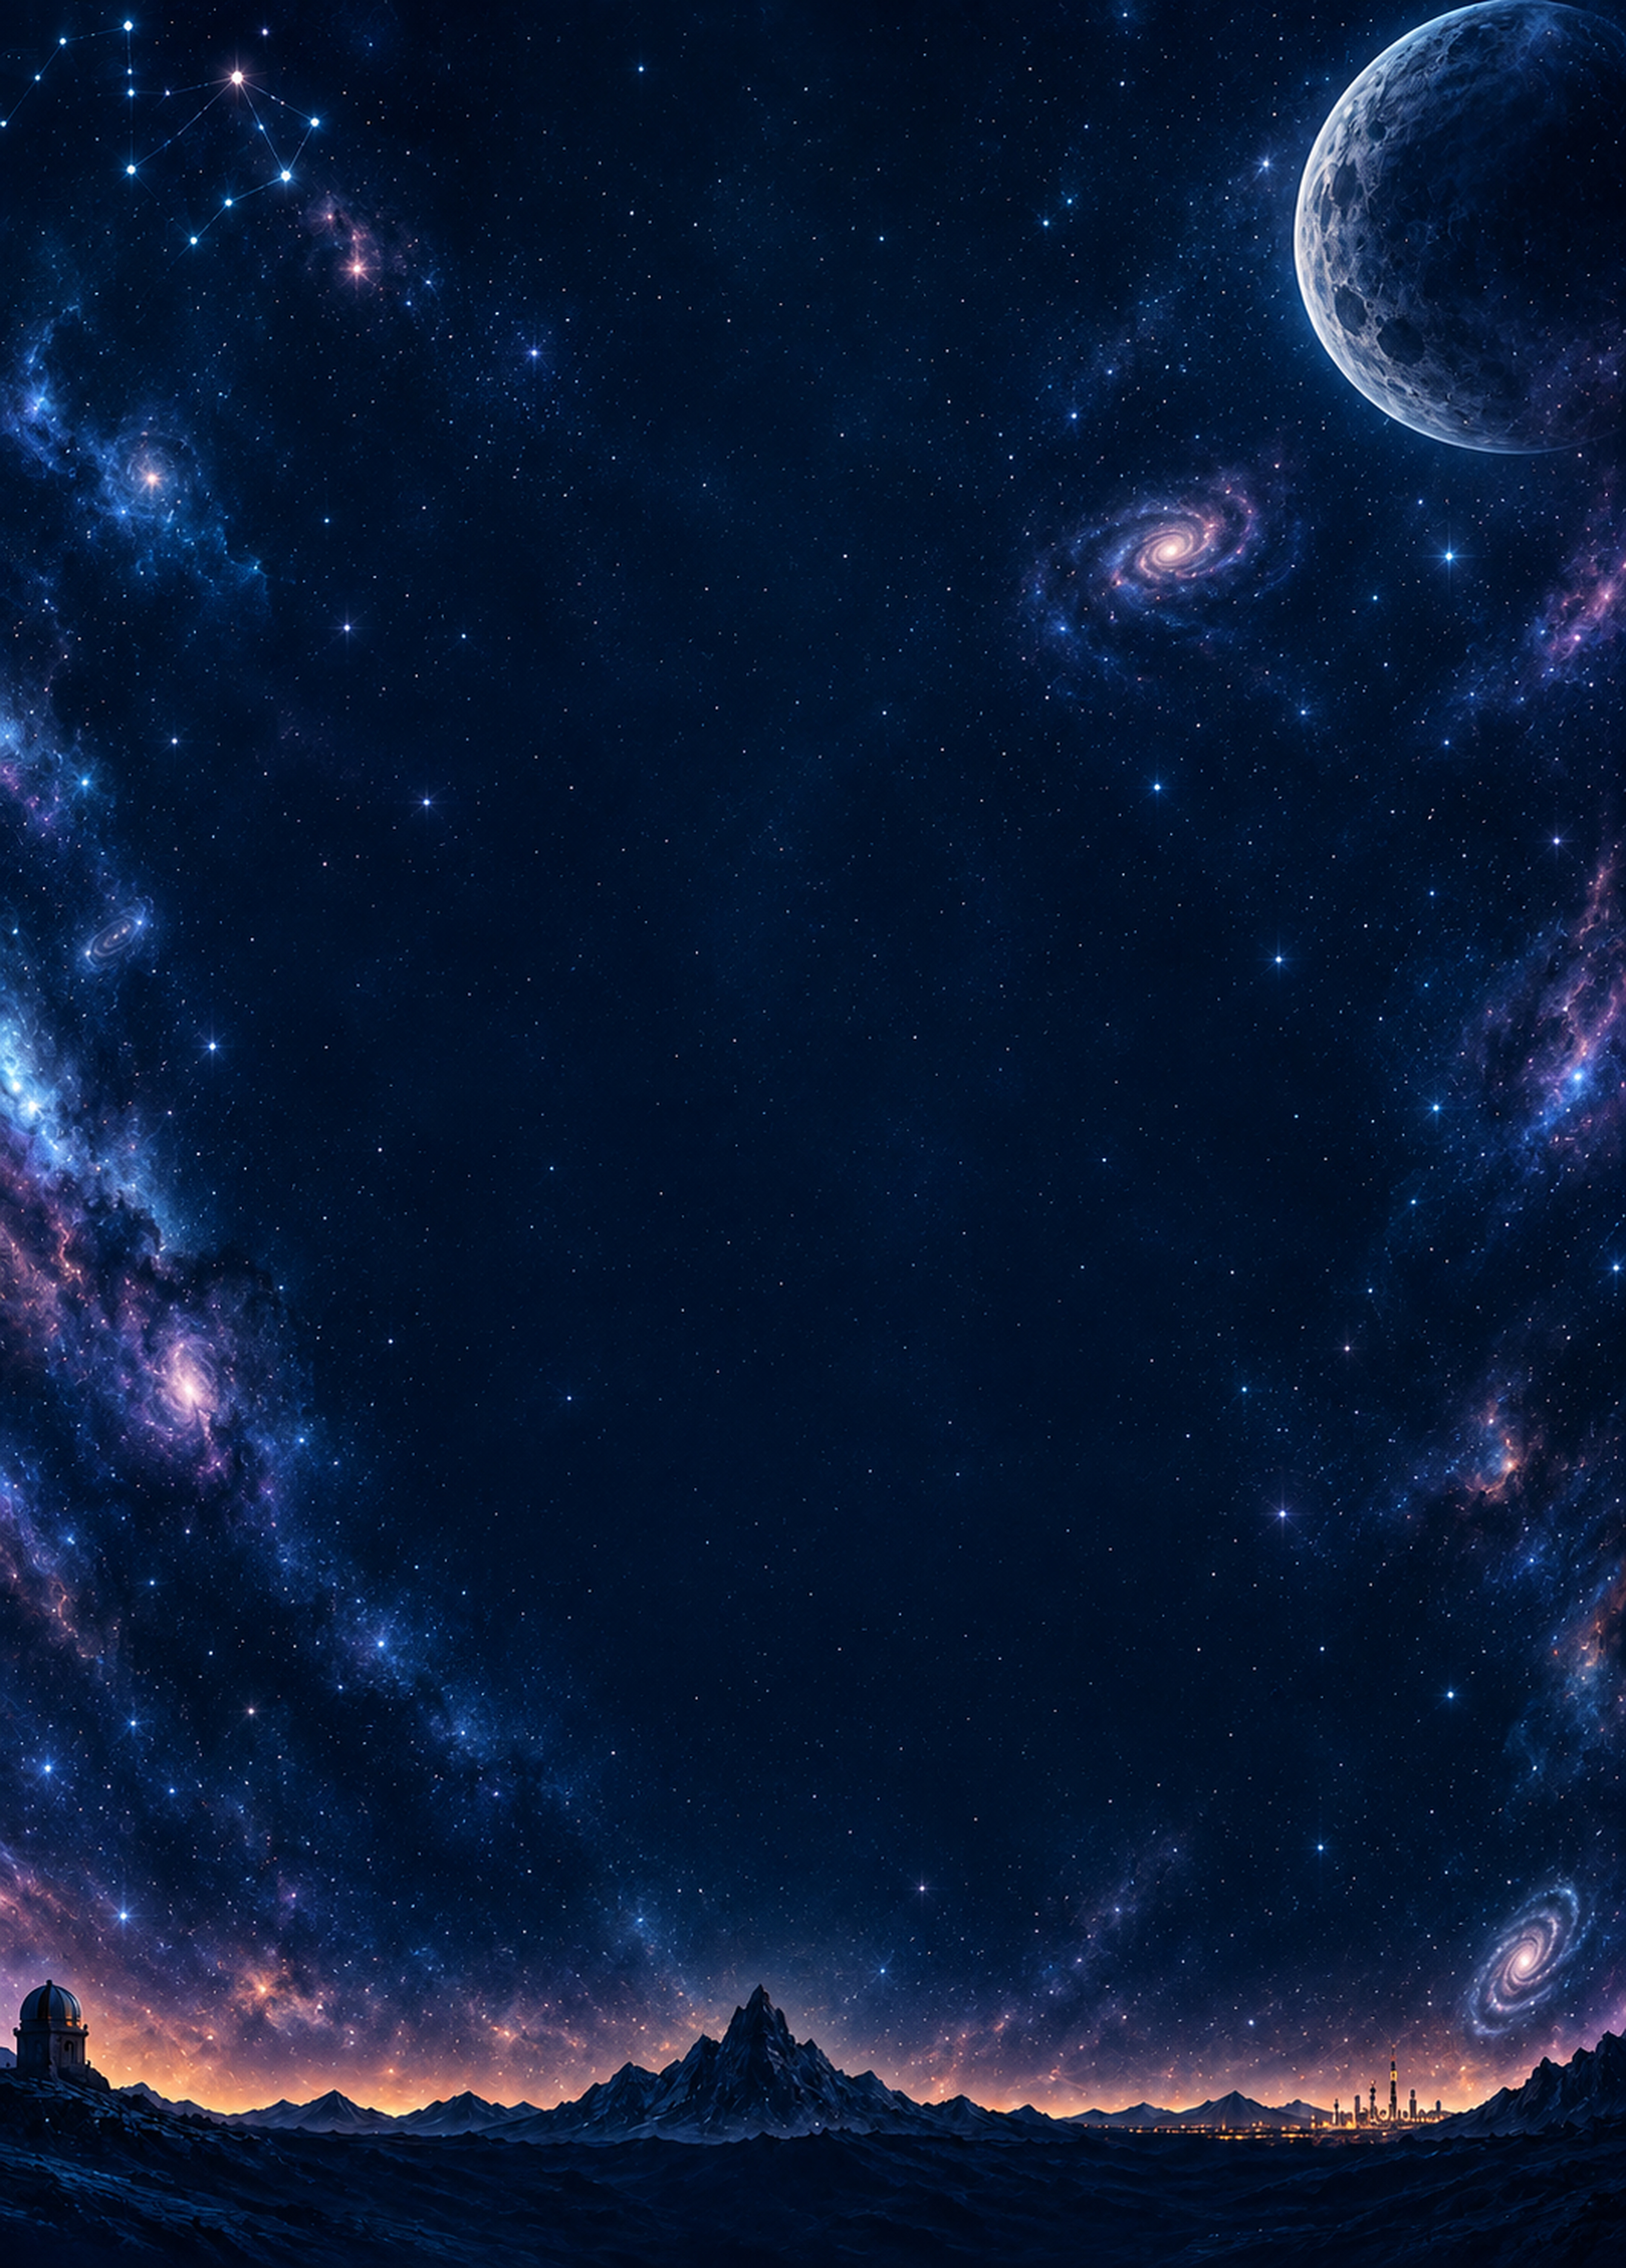
\includegraphics[width=\paperwidth,height=\paperheight]{themes/space/assets/background-print.jpg}};
  \end{tikzpicture}%
}

% ====================
% Header
% ====================

\setbeamertemplate{headline}{%
  \vskip0.65cm
  \leavevmode
  \hbox to \paperwidth{%
    \hspace*{1.45cm}%
    \begin{minipage}[t]{5.6cm}
      \centering
      
\includegraphics[width=4.1cm]{gfx/paper_qr.pdf}\\[-0.05cm]
      {\color{SpaceCream}\small Scan for paper}
    \end{minipage}%
    \hfill
    \begin{minipage}[t]{40.3cm}
      \centering
      {\usebeamerfont{headline title}\usebeamercolor[fg]{headline title}\inserttitle\par}
      \vspace{0.30cm}
      {\usebeamerfont{headline author}\usebeamercolor[fg]{headline author}\insertauthor\par}
      \vspace{0.12cm}
      {\usebeamerfont{headline institute}\usebeamercolor[fg]{headline institute}\insertinstitute\par}
    \end{minipage}%
    \hfill
    \begin{minipage}[t]{8.3cm}
      \centering
      \vspace*{0.20cm}
      
\includegraphics[width=7.6cm]{logos/print-safe/lamarr-logo-negative-transparent.png}
    \end{minipage}%
    \hspace*{1.25cm}%
  }
  \vspace{0.45cm}
}

% ====================
% Glowing content panels
% ====================

\newcommand{\spacespark}{%
  
\begin{tikzpicture}[baseline=-0.55ex,x=1cm,y=1cm]
    \fill[SpaceCream]
      (0,0.55) -- (0.10,0.10) -- (0.55,0) -- (0.10,-0.10) --
      (0,-0.55) -- (-0.10,-0.10) -- (-0.55,0) -- (-0.10,0.10) -- cycle;
    \fill[SpaceCyan,opacity=0.75] (0,0) circle (0.12);
  \end{tikzpicture}%
}

\newcommand{\spaceheading}[1]{%
  \spacespark\hspace{0.30cm}%
  {\usebeamerfont{block title}\color{SpaceCream}#1}%
}

\tcbset{space panel/.style={
  enhanced,
  width=\linewidth,
  colback=SpacePanel,
  opacityback=0.88,
  colframe=SpaceCyan,
  opacityframe=0.90,
  coltitle=SpaceCream,
  colbacktitle=SpacePanel,
  opacitybacktitle=0.92,
  fonttitle=\usebeamerfont{block title},
  title={\spaceheading{\insertblocktitle}},
  titlerule=0.45pt,
  boxrule=0.65pt,
  arc=3.0mm,
  outer arc=3.0mm,
  boxsep=0pt,
  left=0.48cm,
  right=0.48cm,
  top=0.22cm,
  bottom=0.22cm,
  before skip=0.45ex,
  after skip=0.45ex
}}

\setbeamertemplate{block begin}{%
  \begin{tcolorbox}[space panel]
    \usebeamerfont{block body}\color{SpaceCream}\justifying
    \setlength{\parskip}{0.45ex}%
}

\setbeamertemplate{block end}{%
  \end{tcolorbox}%
}

\setbeamertemplate{block alerted begin}{%
  \begin{tcolorbox}[space panel,colframe=SpaceGold]
    \usebeamerfont{block body}\color{SpaceCream}\justifying
    \setlength{\parskip}{0.45ex}%
}

\setbeamertemplate{block alerted end}{%
  \end{tcolorbox}%
}

\setbeamertemplate{itemize item}{\raise0.20ex\hbox{\color{SpaceCyan}$\bullet$}}
\setbeamertemplate{itemize subitem}{\raise0.20ex\hbox{\color{SpaceGold}$\circ$}}
\setbeamertemplate{caption label separator}[period]

\renewcommand{\PosterFeatureBegin}[1]{\begin{block}{#1}}
\renewcommand{\PosterFeatureEnd}{\end{block}}
\renewcommand{\PosterTakeawaysBegin}[1]{\begin{alertblock}{#1}}
\renewcommand{\PosterTakeawaysEnd}{\end{alertblock}}
\renewcommand{\PosterFigureBegin}[1]{\begin{block}{#1}}
\renewcommand{\PosterFigureEnd}{\end{block}}
\renewcommand{\PosterInferenceTree}{themes/space/assets/inference_tree.pdf}

% ====================
% Footer
% ====================

\setbeamertemplate{footline}{%
  \begin{beamercolorbox}[wd=\paperwidth,vmode]{space footer}
    \begin{beamercolorbox}[wd=\paperwidth,ht=0.055cm,dp=0cm]{space footer rule}\end{beamercolorbox}
    \vspace{0.16cm}
    \hbox to \paperwidth{%
      \hspace*{2.8cm}%
      \raisebox{-0.16\height}{
\includegraphics[height=1.30cm]{logos/print-safe/tu-dortmund-logo-claim-de.png}}%
      \hfill
      \raisebox{-0.16\height}{
\includegraphics[height=1.20cm]{logos/print-safe/fraunhofer-iais.png}}%
      \hspace{0.45cm}%
      \raisebox{-0.16\height}{
\includegraphics[height=1.05cm]{logos/print-safe/fraunhofer-iml.png}}%
      \hfill
      \raisebox{-0.16\height}{
\includegraphics[height=2.05cm]{logos/print-safe/uni_bonn-footer.png}}%
      \hfill
      \raisebox{-0.16\height}{
\includegraphics[height=1.70cm]{logos/print-safe/NRWLogo-footer.png}}%
      \hspace{0.65cm}%
      \raisebox{-0.16\height}{
\includegraphics[height=1.90cm]{logos/print-safe/BFTR-footer.png}}%
      \hspace*{2.8cm}%
    }
    \vspace{0.18cm}
  \end{beamercolorbox}%
}
